\mode*

\begin{frame}
\frametitle{The R Package DoubleML:\\ Building Principles}

\begin{block}{DoubleML -  Building Principles}
\footnotesize
\begin{tabular}{l l c}
\multirow{2}{*}{\textbf{Key ingredient}} &\multirow{2}{*}{\textbf{Implementation}} & \multirow{2}{*}{ \pdftooltip{
\includegraphics[width=0.09\textwidth]{pictures_and_logos/DoubleML_Rhino_1000x1000.png}}{The logo of the DoubleML package for R.} } \\ & &  \\ & & \\[-0.8ex]
1. Orthogonal score &  Object-oriented implementation & \multirow{4}{*}{ \pdftooltip{\includegraphics[width=0.07\textwidth]{pictures_and_logos/R6.png}}{The logo of the R6 package for R.} }  \\
                    &  with \texttt{R6}; exploit common structure & \\
                    & centered around a (linear) score  &\\ & function $\psi(\cdot)$ & \\  & & \\[-0.8ex]
2. High-quality ML & State-of-the art ML prediction \& tuning  &  \multirow{5}{*}{ \pdftooltip{
\includegraphics[width=0.08\textwidth]{pictures_and_logos/mlr.png}}{The logo of the mlr3 package for R.} }  \\
                   & methods provided by \texttt{mlr3} ecosystem & \\
                   & (meta packages) &\\  & & \\[-0.8ex]
3. Sample splitting & Built-in resampling schemes of \texttt{mlr3} & \\
\end{tabular}
\end{block}
\end{frame}


\begin{frame}
\frametitle{The R Package DoubleML:\\ Main Dependencies and Installation}
\vspace*{-10pt}
%\begin{columns}[t]
%\begin{column}{0.4\textwidth}
\begin{block}{\pdftooltip{Dependencies}{A box containing the names of the main dependencies of the DoubleML package together with their logos. These are the packages mlr3, R6, data.table, mlr3learners and mlr3tuning.}}
\vspace{8pt}
\begin{columns}[t]
\begin{column}{0.25\textwidth}
\pkgDependency{mlr.png}{\texttt{mlr3}} 
\vspace{8pt}
\pkgDependency{mlr.png}{\texttt{mlr3learners}}
\end{column}
\begin{column}{0.25\textwidth}
\pkgDependency{r6.png}{\texttt{R6}}
\vspace{8pt}
\pkgDependency{mlr.png}{\texttt{mlr3tuning}}
\end{column}
\begin{column}{0.25\textwidth}
\pkgDependency{datatable.png}{\texttt{data.table}} 
\end{column}
\end{columns}
\end{block}
\vspace{10pt}
%\end{column}
%\begin{column}{0.6\textwidth}
\begin{block}{Installation}
\begin{itemize}
\item \textbf{Latest} CRAN \textbf{release} \\
\boxedText{\textcolor{white}{\texttt{\footnotesize \$ install.packages('DoubleML')}}}
\item \textbf{Development version} from GitHub \\
\boxedText{\textcolor{white}{\texttt{\footnotesize \$ remotes::install\_github('DoubleML/doubleml-for-r')}}}
\end{itemize}
\end{block}
%\end{column}
%\end{columns}
\end{frame}


\begin{frame}
\frametitle{Why an Object-Orientated Implementation?}
\begin{itemize}
\item Given the components ($\psi^a(\cdot)$ \& $\psi^b(\cdot)$) of a linear Neyman orthogonal score function $\psi(\cdot)$, a \textbf{general implementation} is possible for
\begin{itemize}
\item The estimation of the \textbf{orthogonal parameters}
\item The computation of the \textbf{score} $\psi(W; \theta, \eta)$
\item The estimation of \textbf{standard errors}
\item The computation of \textbf{confidence intervals}
\item A \textbf{multiplier bootstrap} procedure for simultaneous inference
\end{itemize}
\item The \textbf{sample splitting} can be implemented in general as well
\end{itemize}
$\rightarrow$ Implemented in the \textbf{abstract base class} \texttt{DoubleML}
\begin{itemize}
\item The \textbf{score components} and the estimation of the \textbf{nuisance models} have to be implemented \textbf{model-specifically}
\end{itemize}
$\rightarrow$ Implemented in \textbf{model-specific classes} inherited from \texttt{DoubleML}
\end{frame}


\begin{frame}
\frametitle{Class Structure and Causal Models}
\begin{center}
\pdftooltip{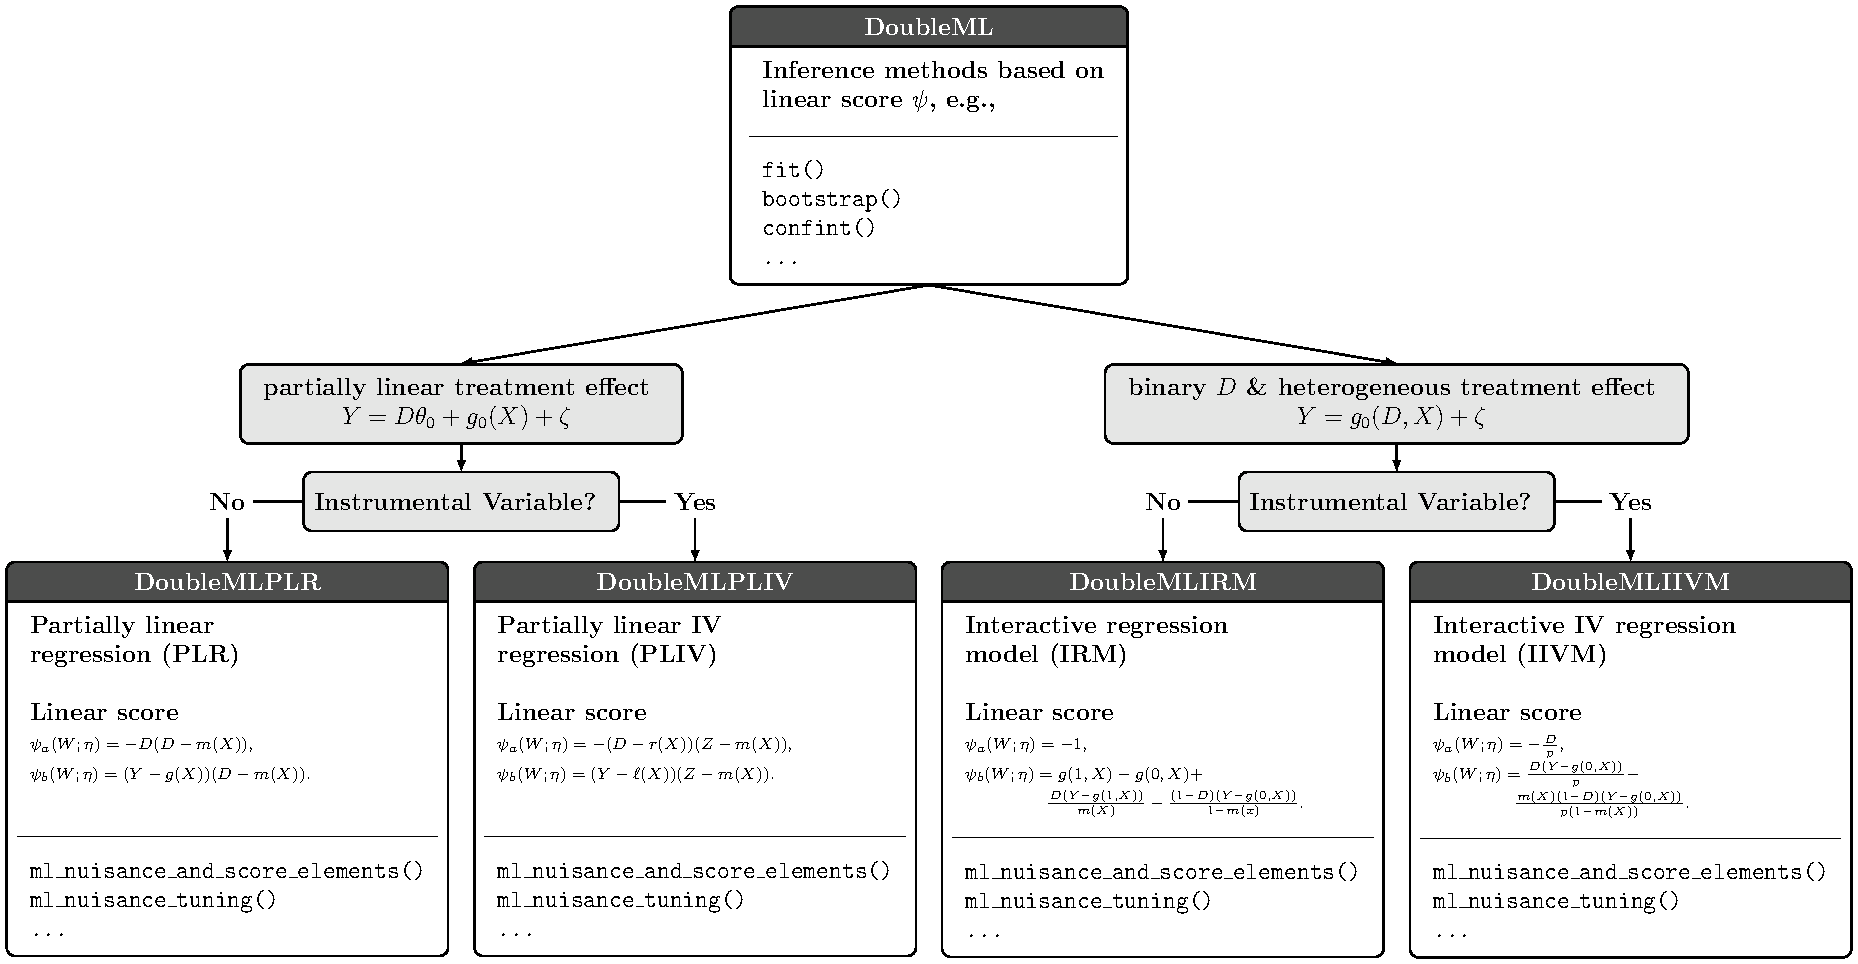
\includegraphics[width = 1\textwidth]{workflow/doubleml_models_with_linear_score_classes_methods.pdf}}{The figure shows a diagramm of the object class structure in DoubleML. On top, there is a box illustrating the base class DoubleML. In this class, inference methods that are based on a linear score function PSI are implemented, for example the methods fit() and confint() for parameter estimation and construction of confidence intervals. Below, there are four different boxes indiciating four different model classes: DoubleMLPLR for partially linear regression models, DoubleMLPLIV for partially linear instrumental variable regression, DoubleMLIRM for an interactive or nonparametric regression  model and DoubleMLIIVM for an IV-version of this interactive regression model. Each of these models is characterized by a different score function PSI.}
\end{center}

\end{frame}


\begin{frame}
\frametitle{Advantages of the Object-Orientation}
\begin{itemize}
\item \texttt{DoubleML} gives the user a \textbf{high flexibility} with regard to the specification of DML models:
\begin{itemize}
\item Choice of ML methods for approximating the nuisance functions
\item Different resampling schemes (repeated cross-fitting)
\item DML algorithms DML1 and DML2
\item Different Neyman orthogonal score functions
\end{itemize}
\item \texttt{DoubleML} can be \textbf{easily extended}
\begin{itemize}
\item New model classes with appropriate Neyman orthogonal score function can be inherited from \texttt{DoubleML}
\item The package features \texttt{callables} as score functions which makes it easy to extend existing model classes
\item The resampling schemes are customizable in a flexible way
\end{itemize}
\end{itemize}

\end{frame}

